%
%  untitled
%
%  Created by Sam Anzaroot on 2012-10-05.
%  Copyright (c) 2012 __MyCompanyName__. All rights reserved.
%
\documentclass[twocolumn,letterpaper]{article}

% Use utf-8 encoding for foreign characters
\usepackage[utf8]{inputenc}

% Setup for fullpage use
\usepackage{fullpage}

% Multipart figures
%\usepackage{subfigure}

% More symbols
\usepackage{amsmath}

% Package for including code in the document
\usepackage{listings}

\usepackage{ifpdf}

\ifpdf
\usepackage[pdftex]{graphicx}
\else
\usepackage{graphicx}
\fi

\usepackage{todonotes}

\setlength{\marginparwidth}{2cm}

\title{Author Linkage in Records using Temporal Information and Conditional Random Fields : A midterm report}
\author{Sam Anzaroot, Jiaping Zheng}

\date{}

\begin{document}

\ifpdf
\DeclareGraphicsExtensions{.pdf, .jpg, .tif}
\else
\DeclareGraphicsExtensions{.eps, .jpg}
\fi

\maketitle

\section{Introduction} % (fold)
\label{sec:introduction}
Record Linking is the task of clustering records in a database such that elements in the same cluster refer to the same real world object. For example, in the DBLP page for David Smith, there are at least three different individuals with publications named David Smith appearing, and the output of a record linker would cluster each David Smith's publications into separate clusters. Various attempts have been made for record linking authors of publications listed in datasets such as DBLP. This task is important because there are many downstream applications that require clean clustering of such information, for example, determining the most prolific authors is only accurate if such clusterings are valid. Network analysis of coauthorship also depends on correct clustering of authors. This task requires a classifer to determine the matchings between two records. This task is not a solved one, and we will attempt to build a more robust classifier.
% section introduction (end)

\section{Related Work} % (fold)
\label{sec:related_work}
\paragraph{Survey of Related work} % (fold)
\label{par:survey_of_related_work}
The research field of record clustering is a very active one. This task is a important one for many different applications, and as such there are many different names for this task. Names include: record clustering, record deduplication, record linking, entity resolution, etc. There are many components to a record linking system. The first are methods of paring down which records are of in need of clustering for efficiency. The task also requires a system for classifying whether or not a set of records match. In addition, methods of effectively clustering supersets of records indepedently classified are neccisary. In order to classify records, effective similarity and/or compatibility measures are needed as features in a classifier. In this report, we are focusing in on building a better classifier for disambiguating authors in DBLP, and generating better features. 
% paragraph survey_of_related_work (end)

Similarity metrics are important for classification as they provide information in which a classifier can make a desicion on. Others have shown that adding temporal information into metrics can enhance the quality of classification \cite{DBLP:journals/fcsc/LiDMS12}. These metrics are weighted by how relevant the metrics are given the distance in time between the two records. This weighting is learned from a set of annotated data.

Various numbers of people have attempted to build classifiers using graphical models that include complex dependencies. For example, ``Multi-Relational Record Linkage'' \cite{Domingos04multi} modeled the record linking problem as a conditional random field which improved f1 performance on a publication deduplication task. In this CRF model, each pair of publication records has a binary latent variable to model whether the records are duplicates.  The observations are modeled using similarity functions.  ``Information nodes'' connect the binary duplication variables and the observation nodes which represent whether the fields of the publication in two records match.

``A Conditional Model of Deduplication for Multi-Type Relational Data'' \cite{Culotta05aconditional} extends the model presented in \cite{Domingos04multi} by making the ``information nodes'' first-class variables in the model.  Binary latent variables that indicate record duplication (both paper and venue) are connected in the CRF to capture the interdependencies between the deduplication results of publications and venues.  For example, equivalent venue records that are merged should result in weights in CRF that also encourage merging of paper records.  To perform inference of finding optimal configurations of the latent variables, the authors converted the model into a weighted undirected graph to find a optimal partitioning.  Learning is approximated by maximizing the product of local marginals using limited-memory BFGS.  Their experiments show that up to a 30\% error reduction in venue deduplication and 20\% in paper deduplication. 
% section related_work (end)

\section{Methodology} % (fold)
\label{sec:methodology}
We model the author linkage problem in a conditional random field.

Conditional random fields (CRFs) are undirected graphical models that encode the conditional probability of a set of unobserved random variables $Y$ given a set of observed variables $X$.  Usually the probability can be factored using independence assumptions.  It can be represented in a graph $G$, where the vertices correspond to the variables $X$ and $Y$.  A potential function $\phi_c$ is defined for every clique $c$ in the graph.  The conditional probability $p(y|x)$ can be expressed as
$$p(y|x)=\frac{1}{Z}\prod_c \phi_c(x_c,y_c),$$
where $Z=\sum_y\prod_c \phi_c(x_c,y_c)$ is a normalization factor.  We assume $\phi_c$ is a log-linear combination of feature functions of the variables in clique $c$, thus
$$\phi_c(x_c,y_c)=\exp\left(\sum_k \lambda_k f_k(x_c,y_c)\right).$$
The model parameters $\{\lambda_k\}$ are learned from training data by maximum likelihood estimation.

Specifically, our CRF structure models the conditional probability of
two author strings referring to the same person given the publication
information.  The unobserved random variables in our model include one
binary variable for each pair of author that indicates whether they
refer to the same person.  We also define latent random variables that
represent the compatibility between the names of the authors, between
the publication venues, between their affiliations, and between their
coauthors.  The observed variables are similarity features
\todo{detail} between author names, venues, affiliations, and
coauthors.  We incorporate temporal information \todo {add decay
  figure} for the publication venue and author affiliation
compatibility variables.  \todo{flesh out, add figure} Intuitively
dissimilar affiliations over a long period of time should have a less
influence on the author linkage dicision than that over a short period
of time. The model is shown in Figure \ref{fig:crf}.

\begin{figure*}
\centering
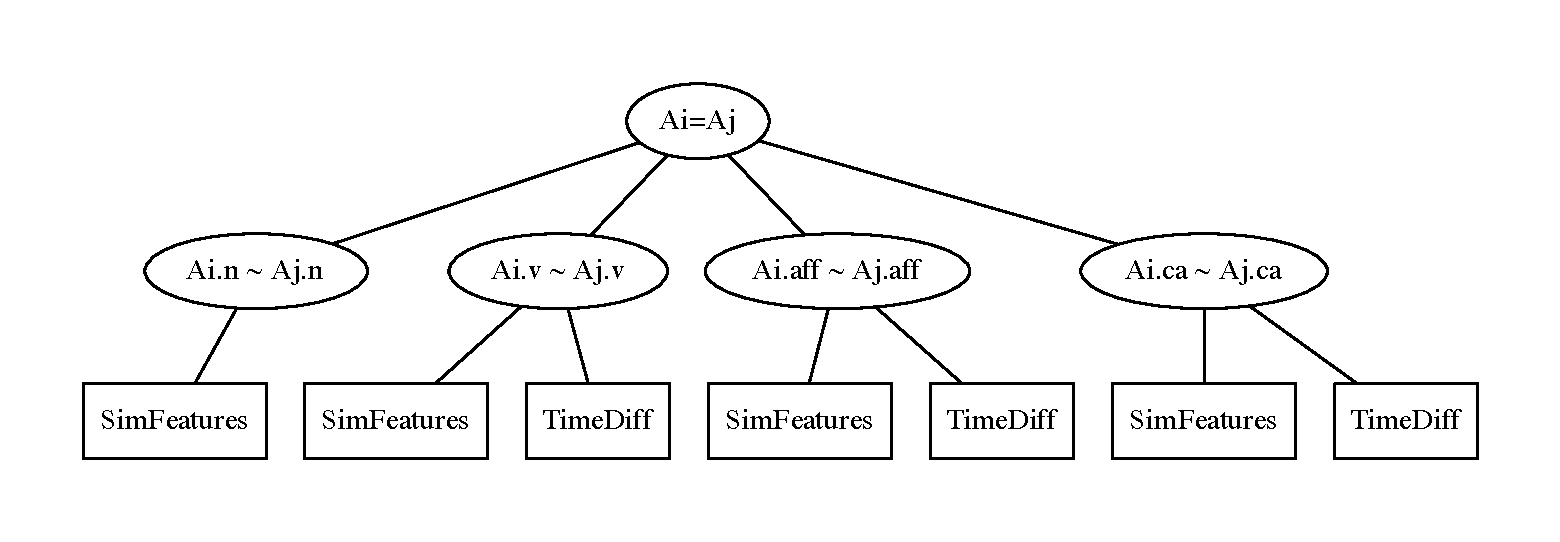
\includegraphics[width=\textwidth]{crf}
\caption{Our CRF model for the author linkage problem.  $A_i$ denotes
  the $i$th author string.  $A_i.n$, $A_i.v$, $A_i.aff$, and $A_i.ca$
  denote the name, venue, affiliation, and coauthors of $A_i$.  The
  oval nodes are unobserved random variables, and the box-shaped ones
  are observed variables.}
\label{fig:crf}
\end{figure*}

\todo{inference, learning, and canopy}

\begin{figure}
\centering
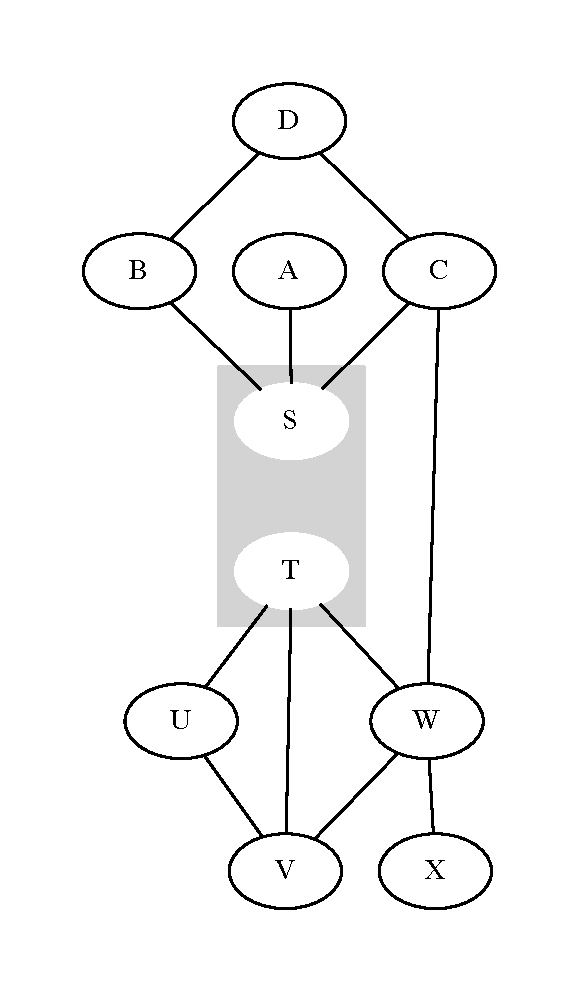
\includegraphics[height=.5\textheight]{coauthor}
\caption{A coauthorship network.  The nodes represent author strings
  in the database.  An edge between two nodes means that the two
  authors coauthored a paper.  $S$ and $T$ are the two author strings
  that the model is predicting to be the same.}
\label{fig:coauthor}
\end{figure}

Unlike the model proposed in Culotta and
McCallum\cite{Culotta05aconditional}, which deduplicates publication
title and venues jointly, our model focuses on author coreference
resolution.  Learning and inference in such a complicated model is
intractable.  However, since the DBLP data is generated directly from
entire conference proceedings and journals, the publication records
are less noisy.  Our model takes advantage of the
reliability of the source data and disambiguates only ambiguous author
information.  Therefore, our model is more scalable one.

Linking pairs of author names is only the first step in the author
linkage problem.  To generate clusters of author names that refer to
the same person, we take the transitive closure of the pairwise
predictions from the CRF model.
% section methodology (end)

\section{Proposed Experiments} % (fold)
\label{sec:proposed_experiments}
In order to show that the model that we propose is better than alternatives, we plan on running numerous experiments. We will compare our completed model with various alternatives. The first is the clustering available already in the DBLP dataset. Those in the DBLP community have tackled the problem by incoperating various heuristics, heavily using coauthorship graphs. They also manually split and combine authors based on human request. We will compare our results to DBLP on some subsection of the DBLP dataset. 

In order to determine the advantages of our model, we will also compare our results with a simple thresholding of our independant similiary functions, and niave combinations thereof. We will generate ROC curves by varying the thresholds. We will compare the best scores of the similarity thesholding for classification with our model.

We will also compare our model with two alternative versions of our model. One will not include any temporal information. One will incoperate temrporal information in our model by performing a simple concatenation of the change in time between the two records and our similarity features. The final model will contain our proposed method of incorperating temporal information. This form of evaluation will inform us of the utitlity of temporal information this domain.
% section proposed_experiments (end)

\section{Evaluation Plan} % (fold)
\label{sec:evaluation}
A simple evaluation metric for our system is the accuracy
of the pairwise prediction from the CRF model.  However, it cannot
reflect the actual performance of the system.  For example, suppose
the system compares the three authors $a_1$, $a_2$, and $a_3$, and the
model predicts that $a_1$ and $a_2$ refer to the same person, $a_2$
and $a_3$ refer to the same person, but $a_2$ and $a_3$ refer to
different people.  The accuracy score would be $2/3$.  However,
computing the transitive closure corrects the wrong classification
prediction.

The author linkage problem is, at its core, a partition of the author
names into clusters, whose members all refer to the same person.  The
coreference resolution problem in natural language processing has the
same character in which textual mentions of real world entities in
documents are clustered into groups that all refer to the same entity.
The community has developed several evaluation metrics that overcome
the problem described above.  These metrics measure how different the
true and predicted partitions are.

We will evaluate our system's performance with two metrics from the
coreference resolution community.  The first is the MUC score
\cite{Vilain95} developed for a coreference resolution shared task.
This metric considers the minimal number of ``links'' between author
strings required to group a set of authors together.

The other metric that we will use is the $B^3$ score \cite{Bagga98b}.
This metric addresses two shortcomings of the MUC score.  MUC score
does not give any credit for separating out singletons (author names
that no other strings refer to), and it treats different errors
indiscriminately (merging two large partitions is equally penalized as
merging smaller partitions).

Evaluating the system on these two metrics provides a balanced view of
the performance.  The MUC score tends to favor larger clusters while
the $B^3$ gives higher penalty to such behavior.  Publications on the
coreference resolution also present multiple scores for this reason.
% section evaluation (end)

\bibliographystyle{plain}
\bibliography{refs}
\end{document}
